\begin{savequote}[75mm] 
It is poor civic hygiene to install technologies that could someday facilitate a police state.
\qauthor{Bruce Schneier} 
\end{savequote}

\chapter{Introduction}

\newthought{online communications} are increasingly opening new possibilities for people to access and create content and interact with one another on the web. On the one hand web application facilitate access to information and foster relationships creation. On the other hand, as networking systems are constantly evolving, and online interactions are becoming more frequent and complex, it is becoming impossible to retain control over what is perceived as our online footprint. More specifically, users can share data with different services, which can subsequently share this information with third parties, sometimes without asking for permission to do so. Third parties are entitled to retain data over time, even if they have no direct connection with the user of the original service. Moreover, it has become a general practice to share content on different platforms and applications simultaneously. Such behaviour creates multiple possibilities for users to be potential targets of various attacks and different profiling activities.

Up to now, in an online context, the right to privacy has commonly been interpreted as a right to \emph{information self-determination}. Acts typically claimed to breach online privacy concern the collection of personal information without consent, the selling of personal information and the further processing of that information. This definition of privacy breach can be considered valid until the user has direct control of the data they have created. This is not always the case. In 2011, the amount of digital information created and replicated globally exceeded 1.8 zettabytes (1.8 trillion gigabytes). 75\% of this information is created by individuals through new media fora such as blogs and via social networks. By the end of 2011, Facebook had 845 million monthly active users, sharing over 30 billion pieces of content~\cite{library-briefing}. Three quarters of the 1.8 trillion gigabytes of digital information online has been created by individual users. On top of that, an increasing amount of additional data about those users is collected by public and private companies, for the most disparate range of uses.

\section{Motivation}

This dissertation is motivated by understanding how data, created by users, flows between applications and services. A very powerful example in this field is the use of federated log in mechanisms. To register to a new social application, users grant them a certain level of access to their identity data, through, for example, their Facebook, Twitter or Google accounts. This data includes details about their identity, their whereabouts and in some situations even the company they work for. Third parties, like Facebook or Google, offer log in technologies, allowing the application to identify the user and receive precise information about them. Once the user grants access to their data, the application stores it and assumes control over how it is further shared. The user will never be notified again on who is accessing their data, nor if these are transferred to third parties. 

\section{Contribution}

In summary, this dissertation makes the following contributions to research within the field of Information Privacy:

\begin{enumerate}
    \item An analysis of how PETs affect recommendation systems for social tagging platforms.
    \item An analysis of privacy risks for proximity based social applications.
    \item An analysis of how users are tracked while surfing the web.
    \item An information theoretic approach to measuring the differential update of the anonymity risk for time variant user profiles.
    \item A hypermedia model of the user online footprint.
\end{enumerate}

Furthermore Fig.~\ref{fig:contributions} illustrates how the contributions listed are mapped to chapters of this thesis.

\begin{figure}
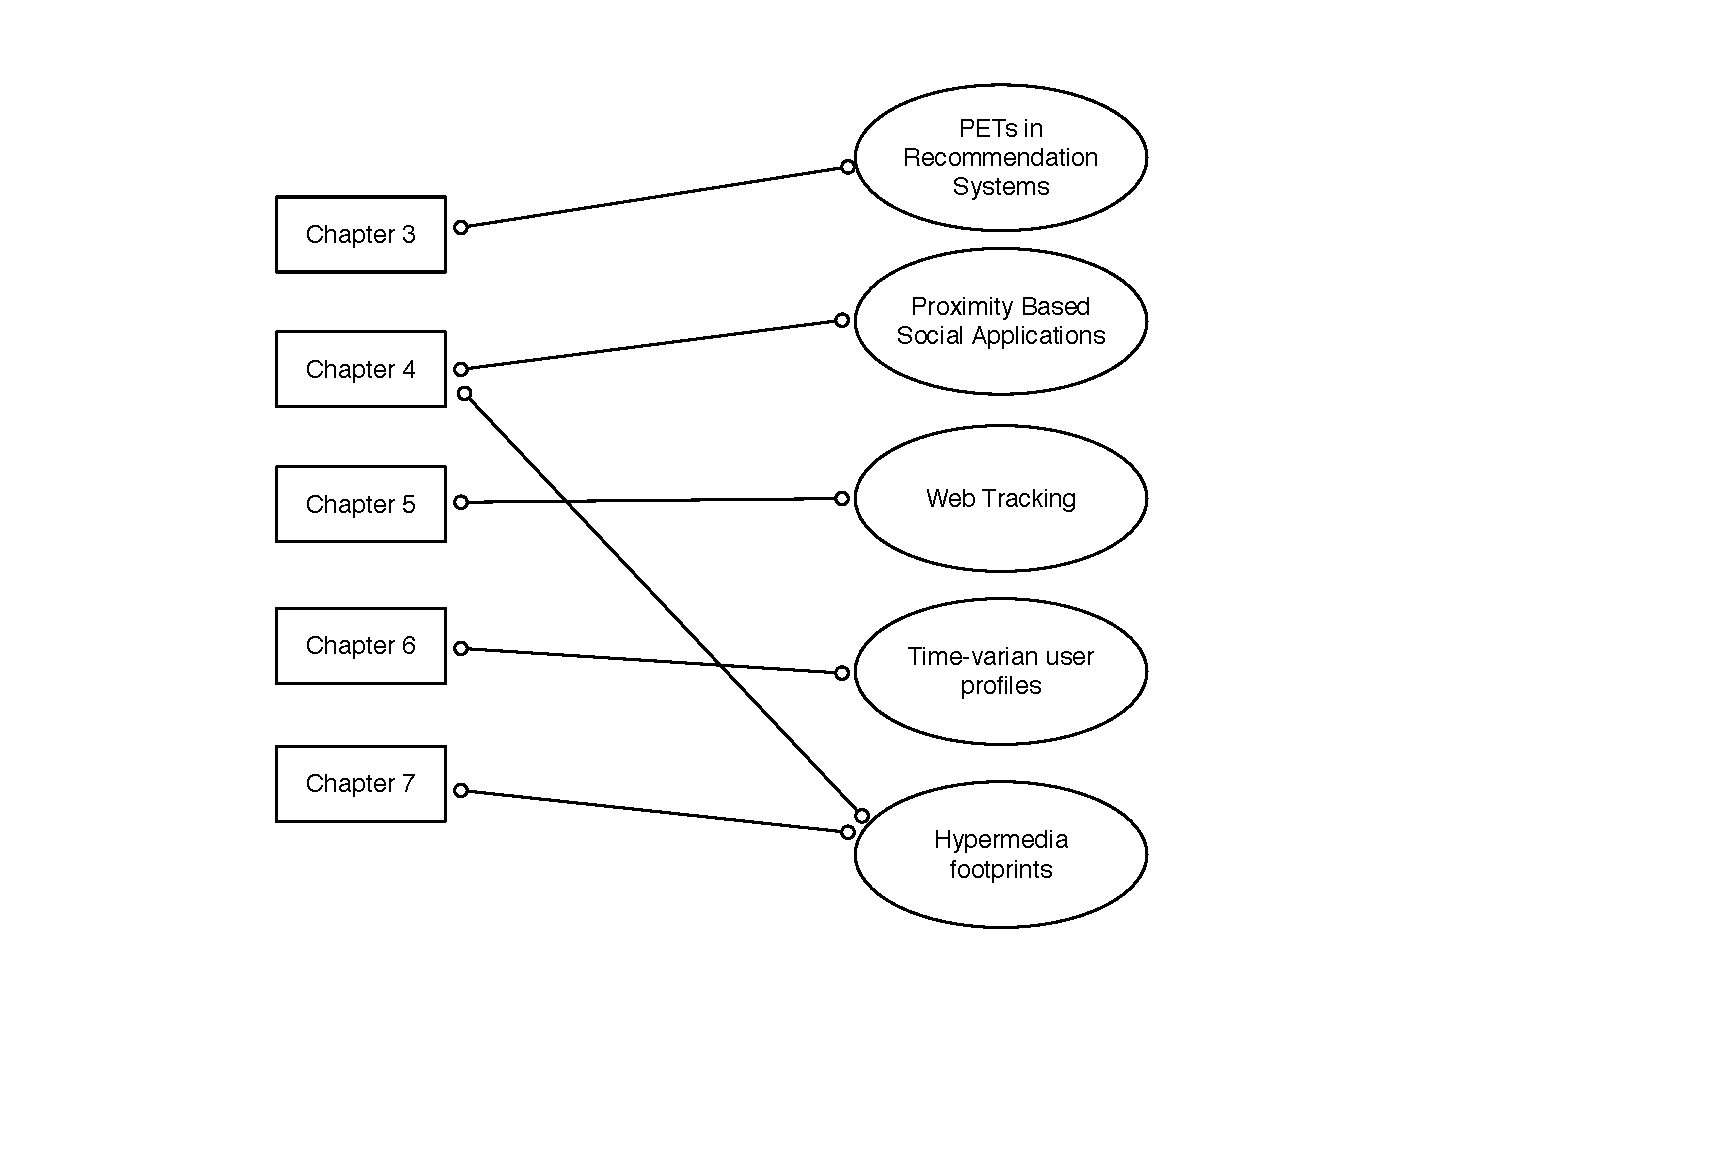
\includegraphics[width=\textwidth]{figures/thesis-map.eps}
\caption[Advertising services feedback loop]{The following image illustrates how contributions are mapped to chapters.}
\label{fig:contributions}
\end{figure}

\section{Related Publications}

Most of the research results presented in this dissertation have been published in journals and conferences. In this section we provide a list of such publications, together with their complete bibliographic information. Further, we include other complementary articles that are not directly related with the research topic of this thesis, but which are especially
significant from the state-of-the-art perspective.

\subsection{Journal publications}
\begin{enumerate}
    \item Puglisi, S., Parra-Arnau, J., Forn\'e, J. and Rebollo-Monedero, D., 2015. \emph{On content-based recommendation and user privacy in social-tagging systems.} Computer Standards \& Interfaces, 41, pp.17-27. \\
    https://doi.org/10.1016/j.csi.2015.01.004
          
    \item Puglisi, S., Rebollo-Monedero, D. and Forn\'e, J., 2017. \emph{On web user tracking of browsing patterns for personalised advertising.} International Journal of Parallel, Emergent and Distributed Systems, pp.1-20. \\
    https://doi.org/10.1109/MedHocNet.2016.7528432
    
    \item Puglisi, S., Rebollo-Monedero, D. and Forn\'e, J., 2017. \emph{On the Anonymity Risk of Time-Varying User Profiles.} Entropy, preprints \\
    https://doi.org/10.20944/preprints201704.0069.v1
\end{enumerate}

\subsection{Conference publications}
\begin{enumerate}

    \item Puglisi, S., Rebollo-Monedero, D. and Forn\'e, J., 2015, August. \emph{Potential mass surveillance and privacy violations in proximity-based social applications.} In Trustcom/BigDataSE/ISPA, 2015 IEEE (Vol. 1, pp. 1045-1052). IEEE. \\
    https://doi.org/10.1109/Trustcom-BigDataSe-ISPA.2015.481
    
    \item Puglisi, S., Rebollo-Monedero, D. and Forn\'e, J., 2015, September. \emph{You Never Surf Alone. Ubiquitous Tracking of Users’ Browsing Habits.} In International Workshop on Data Privacy Management (pp. 273-280). Springer International Publishing. \\
    https://doi.org/10.1007/978-3-319-29883-2\_20
    
    \item Puglisi, S., Rebollo-Monedero, D. and Forn\'e, J., 2016, June. \emph{On Web user tracking: How third-party http requests track users' browsing patterns for personalised advertising.} In Ad Hoc Networking Workshop (Med-Hoc-Net), 2016 Mediterranean (pp. 1-6). IEEE. \\
    https://doi.org/10.1109/MedHocNet.2016.7528432

\end{enumerate}

Finally, we list the complementary publications.

\begin{enumerate}
    \item Puglisi, S., 2015. \emph{RESTful Rails Development: Building Open Applications and Services.} "O'Reilly Media, Inc.". 
    
    \item Puglisi, S., Moreira, \'A.T., Torregrosa, G.M., Igartua, M.A. and Forn\'e, J., 2016. \emph{MobilitApp: Analysing mobility data of citizens in the metropolitan area of Barcelona.} In Internet of Things. IoT Infrastructures: Second International Summit, IoT 360° 2015, Rome, Italy, October 27-29, 2015. Revised Selected Papers, Part I (pp. 245-250). Springer International Publishing. https://doi.org/10.1007/978-3-319-47063-4\_23
\end{enumerate}

\section{Outline}

The focus of this work is exploring the intersection between accurately modelling users' interactions. We are interesting in obtaining a numerical estimation of the impact of certain user’s activities on their privacy. 

The thesis is structured as follows. This first chapter introduces the thesis and its outline.
 
The second chapter presents a literature review of the problems considered throughout this work.

The third chapter introduces an approach to users' profile modelling based on probability mass functions. We continue presenting Privacy Enhancing Technologies in the field of social tagging systems. This chapter is particularly concerned with understanding how recommendation algorithms react to profile perturbation and how the utility of the algorithm is affected.

The fourth chapter is centred on how proximity-based social applications and the idea of serendipitous discovery of interests, places and social connections can be exploited by potential attackers. It is analysed how this services allow users to interact with people that are currently close to them, by revealing some information about their preferences and whereabouts. This information is acquired through passive geo-localisation and used to build a sense of serendipity. Unfortunately, while this class of applications opens different interaction possibilities for people in urban settings, obtaining access to certain identity information could lead a possible privacy attacker to identify and follow a user in their movements in a specific period of time. The same information shared through the platform could also help an attacker to link the victim’s online profiles to physical identities. This chapter is also concerned with the possibilities presented by mobile devices to act as listening sensors and how these could eventually lead to newer privacy attacks.

The fifth chapter is focused on web tracking and how advertising networks are able \emph{to follow} users while they surf the web. This chapter highlights the shift in the evolution of the Internet, from a stage when web sites were just hypertext documents, with no personalisation of the user experience offered, to the web of today, a world-wide distributed system following specific architectural paradigms. Nowadays, an enormous quantity of user-generated data is shared and consumed by a network of applications and services, reasoning upon users expressed preferences and their social and physical connections. Advertising networks follow users’ browsing habits while they surf the web, continuously collecting their traces and surfing patterns. We analyse how user tracking happens on the web by measuring their online footprint and estimating how quickly advertising networks are able to profile users by their browsing habits.

The sixth chapter explores how the user's profile change every time a user publishes a new post or creates a link with another entity, either another user, or some online resource. When new information is added to the user profile, new private data is exposed. This does not only reveal information about single users' preferences, increasing their privacy risk, but can expose more about their network that single actors intended. This mechanism is self-evident on \emph{social networks} where users receive suggestions based on their friends’ activity. An information theoretic approach to measure the differential update of the anonymity risk for time variant users’ profiles is proposed. This expresses how privacy is affected when new content is posted and how much third party services \emph{get to know} about the users when a new activity is shared. We use real Facebook data to show how our model can be applied on a real world scenario.

In the seventh chapter it is presented a hypermedia model of the user online footprint. This model considers the architectural paradigms of the web and applies them to modelling of private information and especially on how this can be exchanged with a certain level of user control. We analyse the current models to grant access to private data and how this could be modified in order to achieve a better user supervision over their footprints. Furthermore, we analyse how this data could be applied with user willing to grant access to third-party apps to their Facebook profile in exchange for some service.